%
% File naacl2019.tex
%
%% Based on the style files for ACL 2018 and NAACL 2018, which were
%% Based on the style files for ACL-2015, with some improvements
%%  taken from the NAACL-2016 style
%% Based on the style files for ACL-2014, which were, in turn,
%% based on ACL-2013, ACL-2012, ACL-2011, ACL-2010, ACL-IJCNLP-2009,
%% EACL-2009, IJCNLP-2008...
%% Based on the style files for EACL 2006 by 
%%e.agirre@ehu.es or Sergi.Balari@uab.es
%% and that of ACL 08 by Joakim Nivre and Noah Smith

\documentclass[11pt,a4paper]{article}
\usepackage[hyperref]{naaclhlt2019}
\usepackage{times}
\usepackage{latexsym}

\usepackage{graphicx}
\usepackage{url}

\usepackage{booktabs}
\usepackage{lscape}
\usepackage{amsmath}
\usepackage{amsfonts}
\usepackage{indentfirst}
\usepackage{latexsym}
\usepackage{multirow}
\usepackage{epstopdf}
\usepackage{tabls}
\usepackage{wrapfig}
\usepackage{supertabular}
%\usepackage{subeqn}
\usepackage{subfigure}
\usepackage{enumitem}
\usepackage{natbib}
\usepackage{xspace}
\usepackage{booktabs}
\usepackage{tikz}

\newcommand{\mixer}{\textsc{Mixer}\xspace}
\newcommand{\utility}{\textsc{Utility}\xspace}
\newcommand{\bleu}{\textsc{Bleu}\xspace}
\newcommand{\rouge}{\textsc{Rouge}\xspace}
\newcommand{\meteor}{\textsc{Meteor}\xspace}
\newcommand{\diversity}{\textsc{Diversity}\xspace}
\newcommand{\reinforce}{\textsc{Reinforce}\xspace}
\newcommand{\U}{\mathbb{U}}

%\aclfinalcopy % Uncomment this line for the final submission
%\def\aclpaperid{***} %  Enter the acl Paper ID here

%\setlength\titlebox{5cm}
% You can expand the titlebox if you need extra space
% to show all the authors. Please do not make the titlebox
% smaller than 5cm (the original size); we will check this
% in the camera-ready version and ask you to change it back.

\newcommand\BibTeX{B{\sc ib}\TeX}

\title{Specificity-Controlled Clarification Question Generation Model}

\date{}

\begin{document}
\maketitle
\begin{abstract}

\end{abstract}

\section{Introduction}

In the last chapter, we saw how we can train a sequence-to-sequence neural network model to generate a useful question given an under-specified context. 
We used answer-based adversarial training strategy to train the sequence-to-sequence model. One of our key findings was that an adversarially trained model generates questions that are more specific to the context compared to a model trained using the traditional maximum-likelihood training objective.
Generating questions with a desired level of specificity can be useful in many scenarios.
For instance, consider an automated agent assisting a human in a technical issue through a dialogue. 
At the start of the conversation, we would want the automated agent to ask the human more generic questions in order to understand the general domain of the problem. Whereas, at a later stage of the conversation, we would want the agent to ask more specific questions to narrow down the problem. 
In the e-retail scenario considered in this dissertation,  if the given description belongs to a product which is similar to several other products that currently exist in the dataset, then we might want our automated system to generate more specific questions (since we could easily generate generic questions for this product by retrieving the top-K frequently asked questions in the dataset, for instance).
On the other hand, if the given product belongs to a fairly new category, then we might want our system to generate more generic questions. 
In this chapter, therefore, we propose to build a model that given a context and a level of specificity (specific or generic), generates a question with that level of specificity.
For instance, in \autoref{fig:amazon_style_cqa}, given a product description (context) and a level of specificity as ``$<$generic$>$'', our goal is to generate a question such as \textit{``Where was this manufactured?''} which is applicable to many products on amazon.com. 
Whereas, given the same product description and the level of specificity as ``$<$specific$>$'', we would like to generate a question that is more specific to the given product such as \textit{``Is this induction safe?''}

\begin{figure*}[h]
	\fbox{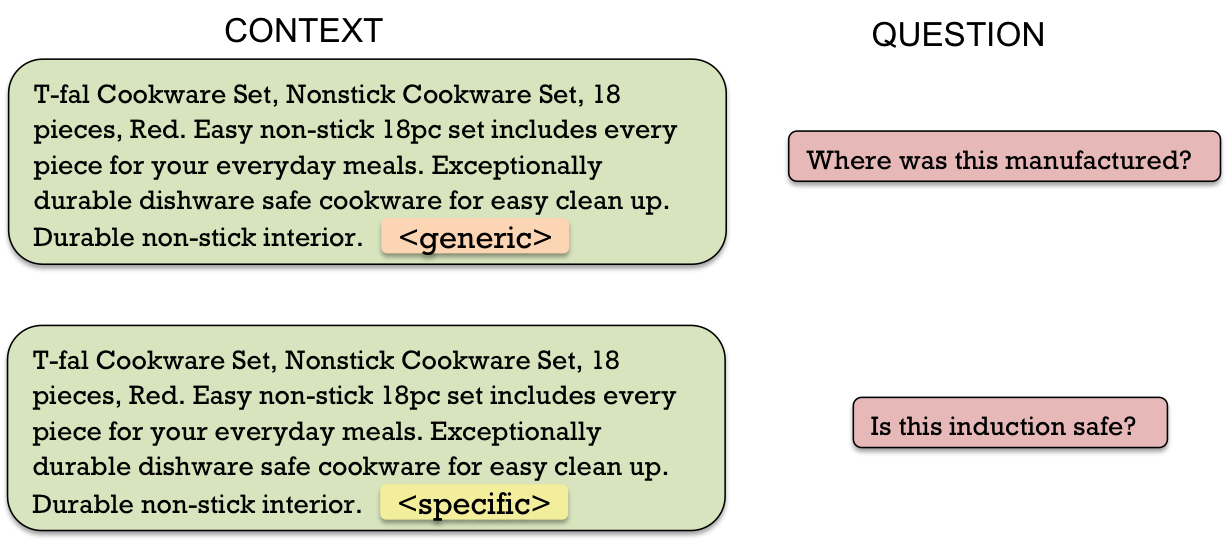
\includegraphics[width=\textwidth]{amazon_style_example}}
    \caption{Sample product description from amazon.com paired with a generic and a specific clarification question.}\label{fig:amazon_style_cqa}
\end{figure*}

We take a semi-supervised approach to our problem of generating specificity controlled questions. Motivated by Sennrich et al. \cite{sennrich2016controlling}, we build a question generation model that incorporates the level of specificity as additional input signal during training\footnote{Sennrich et al. \cite{sennrich2016controlling} refer to this as side constraints.}. In our work, we hypothesize that at training time if we append the context (source) with the level of specificity of the question (target), then the model will learn how to generate questions that at a given level of specificity. In \autoref{fig:style_clarification_roadmap}, the question generation model is trained using context appended with specificity as input and question as the output. In order to do this training, we would need to label all the questions in our training data with their level of specificity i.e. generic vs specific. Doing this labeling manually for the entire training dataset of approximately 150K questions would be too expensive. Hence, we train a supervised model that can learn to automatically label a question (given a context) with its level of specificity to the given context. \autoref{fig:style_clarification_roadmap} shows our specificity classifier trained using a relatively small set of questions manually annotated with their level of specificity. 

\begin{figure*}[t]
	\fbox{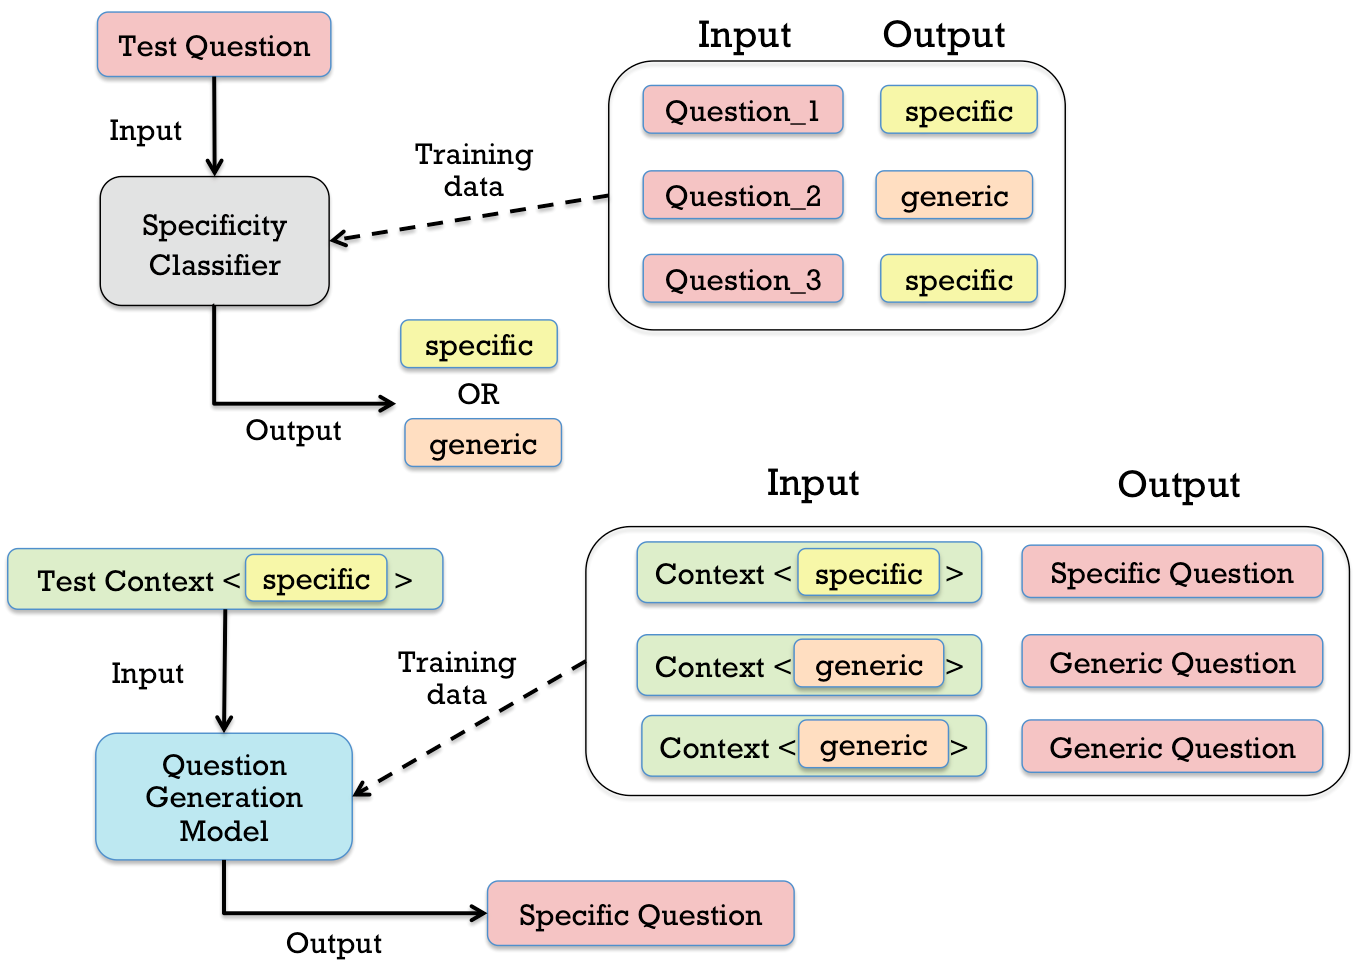
\includegraphics[width=\textwidth]{style_clarification_roadmap}}
    \caption{Specificity-controlled question generation model.}\label{fig:style_clarification_roadmap}
\end{figure*}

Our specificity classifier is inspired by the model introduced by Louis and Nenkova \cite{louis2011automatic} who train a binary classifier to automatically identify generic vs specific sentences in news articles. 
Their classifier is based on features that capture lexical and syntactic information, as well as specificity and word polarity. 
They use human annotators to manually annotate a set of sentences with generic/specific labels and train a binary classifier using a logistic regression model. 
Following their work, we use crowdsourcing to annotate a set of 3000 questions from the Amazon dataset with their level of specificity to the product description. 
We use this annotated data to train a binary classifier to predict the level of specificity of a question, given a context. 
We use some of the features introduced by Louis and Nenkova \cite{louis2011automatic} and introduce new features that are indicative of the specificity level of the question to train our binary classifier.

We use our specificity classifier to append the context with the level of specificity of the target question. 
We finally retrain the question generation model described in the previous chapter with the modified context. 
At test time, given a context appended with a level of specificity (generic or specific), our model generates a clarification question at that level of specificity. 
%\autoref{fig:amazon_style_cqa} shows two example (context, question) pairs. The first context is appended with the ``generic'' tag since the question paired with it is a generic question, whereas the second context is appended with the ``specific'' tag since the question paired with it is a specific question.  

\section{Related Work}

We consider specificity as a dimension of style. Sociolinguistics defines style as a set of linguistic variants with specific social meanings. 
Hovy \cite{hovy1987generating} argues that by varying the style of a text, people convey more information than is present in the literal meaning of the words.
In order to build automated intelligent agents that can effectively communicate with humans, it is important that we teach these agents to recognize the various stylistic variations in human language and also teach them to generate language in a particular given style. 
In the field of natural language processing, there has been previous work on both identifying style and generating text in a given style. 

Under style identification, there has been work on detecting formality of a given text at the lexical level \cite{brooke2010automatic,lahiri2011informality,brooke2014supervised,pavlick2015inducing}, at the sentence level \cite{pavlick2016empirical} and at the document level \cite{sheikha2010automatic,peterson2011email,mosquera2012smile}. 
Markowitz and Hancock \cite{markowitz2016linguistic} studied writing styles in fraudulent papers whereas Feng et al. \cite{feng2012syntactic} build models for deception detection. 
Danescu-Niculescu-Mizil et al. \cite{danescu2013computational} proposed a framework for identifying linguistics aspects of politeness. 
Koppel et al. \cite{koppel2002automatically,koppel2009computational,koppel2011authorship} develop machine learning models for authorship identification, where the style corresponds to the writing style of an author. 
Previous work most relevant to us is the work around detecting generic/specific distinctions of text. Reiter and Frank \cite{reiter2010identifying} introduce a method for distinguishing between noun phrases that describe class of individuals (generic) versus those that refer to specific individuals. 
Mathew and Katz \cite{mathew2009supervised} distinguish between sentences that relate to specific event versus those that relate to general facts. 
Louis and Nenkova \cite{louis2011automatic} build a model to automatically identify general and specific sentences motivated by potential applications
in summarization and writing feedback.

Generating style-controlled text has been studied in three different settings before: supervised learning, semi-supervised setting and unsupervised setting.
Under supervised setting, Xu et al. \cite{xu2012paraphrasing} develop a statistical machine translation based model for paraphrasing sentences into Shakespearean English whereas 
Jhamtani et al. \cite{jhamtani2017shakespearizing} develop a neural machine translation based model for the same task. 
Recently, we \cite{RaoT18} developed models for automatically rewriting sentences from informal to formal style and vice-versa. 
Under semi-supervised setting,  Sennrich et al. \cite{sennrich2016controlling} develop models to control politeness of the generated text using side constraints where the source is appended with an artificial token denoting the style in which we want the model to generate its target. Yamagishi et al. \cite{yamagishi2016controlling} use a similar idea for controlling the voice of the generated text. 
Niu et al. \cite{niu2017study,niu2018multi} control formality during translation. 
Under unsupervised setting, Hu et al. \cite{hu2017toward} control the sentiment and the tense of the generated text by learning a disentangled latent representation in a neural generative model. 
Ficler and Goldberg \cite{ficler2017controlling} control several linguistic style aspects simultaneously by conditioning a recurrent neural network language model on specific style (professional, personal, length) and content (theme, sentiment) parameters. 


\section{Annotating Questions with Specificity Level}

The key idea behind the use of side constraints is to guide a model to generate text constrained with a certain linguistic phenomena by training it on sentences that have been annotated with such constraints. In our scenario, the constraint is the level of specificity. More specifically, our input is the context and the output is the question as the per the specified level of specificity. Hence, while training this model we need to append the source i.e. the context with the level of specificity of the target i.e. the question. Given that our neural network based question generation model requires huge amounts of training data, annotating the entire training data  (around 100K questions) with the level of specificity manually would be too time consuming and costly. Therefore, we take a machine learning approach to this problem where we annotate a subset of the training data using humans and train a machine learning model on this annotated data which learns to predict the level of specificity of a question given the context. In this section, we describe how we collect human annotations on the subset of the training data. 

\subsection{Annotation Design}

We define our annotation task as given a context and a clarification question, annotate if the question is generic or specific to the given context. One obvious way to do this task would be to show the annotators the context and the question and ask them to choose between generic or specific. However, we found that doing this annotation task for a question (given a context)  without knowing the other questions asked to that context is really hard and unintuitive. We found that an easier task would be to compare the level of specificity of two questions given a context. For instance, given the context in \autoref{fig:amazon_example}, annotating the level of specificity of the question  ``Are they ok for induction stove?" in isolation is difficult. However, comparing the specificity level of this question with say another question ``Where are they made?" is easier, we can say that the former question is more specific than the latter since the latter is applicable to a larger set of products.  Hence, we design an annotation scheme where given a context and two questions Question A and Question B, we ask annotators to compare the level of specificity of the two questions by choosing from the following options:\\
1. Question A is more specific \\
2. Question B is more specific \\
3. Both questions are at the same level of specificity\\
Each question pair is annotated by five annotators. 
We use Figure-Eight \footnote{\url{https://www.figure-eight.com/}}, a crowdsourcing platform, to collect these annotations. Each pair of questions is annotated by five annotators. 


\subsection{Getting Specificity Levels from Annotations}

The next step would be how to convert these comparisons into individual generic/specific labels for the questions. Given a context and the $N$ questions asked to that context, we collect annotations such that each question is compared to $K$ other questions in the set $N$. Each question pair $(q_i, q_j)$ is annotated by five annotators. The platform we use to collect annotations assigns a trust value to each of its annotators based on the number of annotations performed by the annotator and how well the annotator performed on the test questions. This trust value is between 0 and 1. We calculate the specificity score for each question as \\

$ \textnormal{specificity\_score}(q_i) = \frac{1}{K} \sum_{j=1}^K \frac{1}{5} \sum_{a=1}^5 t_a * d_a(i, j) $ \\

where $t_a$ is the trust of the annotator $a$ who annotated the question pair $(q_i, q_j)$, \\
$d_a(i, j) = 1$; if annotator $a$ annotated $q_i$ as more specific than $q_j$, \\
$d_a(i, j) = -1$; if annotator $a$ annotated $q_j$ as more specific than $q_i$, \\
$d_a(i, j) = 0$; if annotator $a$ annotated $q_i$ is at the same level of specificity as $q_j$ \\

The specificity score calculated as above is a value between -1 and 1. Given this value, we set a threshold $S$ and when the score for a question is less than $S$, we label it as generic whereas when it is greater than or equal to $S$, we label it as specific. We set a global threshold of $S = 0$ for all contexts. 

If we collect annotations such that each question is compared to every other questions in the set of $N$, then we could get a more accurate specificity score for a question. However, given that $N$ can be as high as 10, collecting $\frac{N(N-1)}{2}$ annotations per context could be expensive. We, therefore, collect annotations such that each question is compared to two other questions in the set $N$. 

To ensure that this method is reliable, for 25 of the contexts, we collect annotations such that each question is compared to every other question in the set $N$. On this subset, we calculate the specificity scores of the questions using $(N-1)$ comparisons per question ($S_{\textnormal{all\_comparisons}}$) and we calculate the specificity scores of the questions using two comparisons per question ($S_{\textnormal{two\_comparisons}}$). In order to understand how much do the specificity scores vary when they are calculated using these two different methods, we calculate the accuracy of the $S_{\textnormal{two\_comparisons}}$ scores over the $S_{\textnormal{all\_comparisons}}$ scores. We get an accuracy of 0.89 suggesting that, although the scores calculated using two comparisons can be noisy, they do not deviate too much from those obtained using all comparisons. 

\section{Model for Automatically Predicting Specificity Level}

Given the specific/generic annotations on a subset of our training data, our next step is to train a machine learning model that can learn to predict the specificity level given a context and a question. Louis and Nenkova  \cite{louis2011automatic} introduce a supervised classifier for automatically predicting whether a sentence in a summary is generic or specific. They define specificity as the level of detail present in a given sentence. The definition of specificity in our setting is how specific the question is to the given context.  Their classifier is based on lexical and syntactic features. We use some of the features described in their work and introduce some new features relevant to our setting to create a similar classifier that predicts the level of specificity of a question given its context. The features used in our model are described below: \\

\noindent \textbf{Question Length.} Generic questions tend to be shorter in length compared to specific questions. For instance, ``What are the dimensions?'', ``What is the size of the pillow?'' are shorter in length compared to questions like ``Does this pillow have a zipper or does it come with a cover?''. We count the number of words in the question and use the count as a feature. Additionally, we use a part-of-speech tagger to tag the words in the question and count the number of nouns in the question and use that as feature. These two features were used by Louis and Nenkova \cite{louis2011automatic} in their model as well.\\

\noindent \textbf{Path in WordNet.} Questions that are more specific to a context tend to have more specific words. Resnik \cite{resnik1995using} uses the hypernym relations in WordNet \cite{miller1990introduction} to compute the specificity of a given word. Motivated by this idea, we compute the length of the path of every noun and verb in a question to the root of WordNet tree through hypernym relations. Longer paths would indicate that the words are more specific. Similar to Louis and Nenkova \cite{louis2011automatic}, we use the average, min and max values of these lengths and use them as features. \\

\noindent \textbf{Inverse Document Frequency.} Another way to identify specific words is to calculate its inverse document frequency (IDF). IDF of a given term is defined by the inverse of the number of documents that contain that term. More formally $\textnormal{IDF}(w) = \log (\frac{1}{\text{count of docs containing } w })$. In our setting, we consider a product description to be a document. So the IDF of a word in a given question is defined by the inverse of the counts of product descriptions that contain that word. We calculate the IDF for every word in the question and include the maximum IDF, the minimum IDF and the average IDF as features. This feature is similar to the one used by Louis and Nenkova \cite{louis2011automatic}  except that instead of calculating the document frequency over New York Times articles, we calculate the document frequency over product descriptions\\

\noindent \textbf{Syntax.} Similar to Louis and Nenkova \cite{louis2011automatic}, we find that the use of nouns, adjectives and cardinals are good indicators of specificity. For instance, more specific questions tend to use more proper nouns, adjectives and cardinals (numbers). We use parts-of-speech tagger to tag the words in the questions and include the counts of proper nouns (NNP), adjectives (ADJ) and cardinals (CD) as features. \\

\noindent \textbf{Polarity.} Louis and Nenkova \cite{louis2011automatic} find that word polarity can be strong indicator of the level of specificity. For instance, strong opinions are indicative of generic sentences. To identify positive, negative and polar words, they use The General Inquirer and the MPQA Subjectivity lexicons. 
We find that these two lexicons, which mainly contain words frequently appearing in news articles,  are less relevant for us due to the different nature of our dataset. 
Hence, we use the Linguistic and Word Inquiry (LIWC)\footnote{\url{http://lit.eecs.umich.edu/~geoliwc/LIWC_Dictionary.htm}} \cite{pennebaker2001linguistic} instead. We use the dictionary category of words in the question as features. Specifically, we consider the following categories under cognitive processes: \textit{insight, causation, discrepancy, tentative, certainty, differentiation}. For each of these categories, we count the number of words in question that belong to that category and include that as a feature. \\

\noindent \textbf{Question bag-of-words.} We define a vector of the size of the vocabulary over the words in all the questions of our train set. Given a question, we set all the word positions that are included in the question to one in the vector and set the remaining to zero. We include this vector as a feature. This is similar to the ``lexical (words)'' features used by Louis and Nenkova \cite{louis2011automatic}. \\

The features described above were adapted from Louis and Nenkova \cite{louis2011automatic}. We now describe the new features we introduced specifically for our problem. \\

\noindent \textbf{*Average word embeddings.} We train GloVe \cite{pennington2014glove}, a word embedding model, on all contexts and questions in our Amazon dataset. We compute an average over the word embeddings of all the words in the question ($\bar{q}$) and include it as a feature. Likewise, we compute an average over the word embeddings of all the words in the context ($\bar{c}$) and include it as a feature.\\

\noindent \textbf{*Similarity to context using word embeddings.} Louis and Nenkova \cite{louis2011automatic} define generic/specific based on the level of detail present in a sentence in isolation. In contrast, the specificity in our setting is measured by how specific is the question to the given context. Hence, we find that the similarity between the question and the given context to be a useful indicator of specificity. We measure this similarity using two ways. In the first way, we measure the similarity between the context and the question in the vector semantic space. We compute an average over the word embeddings of all the words in the context ($\bar{c}$). Similarly, we  compute an average over the word embeddings of all the words in the question ($\bar{q}$). We calculate the cosine similarity between $\bar{c}$ and $\bar{q}$ and use it as a feature. \\
 
\noindent \textbf{*Similarity to context using WordNet.} In the second way, we measure the similarity in the WordNet space. Similar to the path in WordNet feature described previously, we look at the hypernym relation path of every word in the question and every word in the context and count the number of hypernyms that were common in the two paths. We do this for every word pair $(w_q, w_c)$ where $w_q$ is a word in the question and $w_c$ is the word in the context and use the aggregate count as a feature. \\

%\noindent \textbf{Language Model}

Given these features, we train a logistic regression model to make a binary prediction (-1: generic, 1: specific) given a context and a question. We use the Adam \cite{kingma2014adam} optimizer. We use $L2$ regularizer. 

\section{Specificity-Controlled Question Generation Model}

We use the specificity classifier described in the previous section to label all the questions in the training (and tune) data with generic/specific labels. 
We use these labels to append each context with the \textit{$<$specific$>$} tag when the question paired with the context is labeled as specific and with the \textit{$<$generic$>$} tag when the question paired with the context is labeled as generic.
We use this specificity annotated training data to train two specificity-controlled question generation model:\\

\noindent \textbf{Specificity-MLE}: Similar to the \textbf{MLE} model in the previous chapter, we train a sequence-to-sequence learning model \cite{sutskever2014sequence} on (context+specificity, question) pairs using maximum likelihood objective (\autoref{sec:seq2seq}). \\

\noindent \textbf{Specificity-GAN-Utility}: This is the full question generation model described in previous chapter which we train using (context+specificity, question) pairs instead of (context, question) pairs. 
We first pretrain a question generator on (context+specificity, question) pairs and an answer generator model using (context+specificity+question, answer) pairs using maximum likelihood objective. 
We then fine tune the question generator model using \utility function based GAN training (\autoref{sec:gan}) including the \utility discriminator, a \mixer question generator. \\
 
At test time, we predict the specificity level of the target question using our specificity classifier and append the tag corresponding to that label to the context. 

\section{Experimental Results}

\subsection{Specificity Classifier Results}

\begin{table*}[t]
\centering
\begin{tabular}{lcc}
\toprule
Features & Train Accuracy & Test Accuracy \\
\midrule
Question length & 0.55 & 0.55 \\
Path in WordNet & 0.63 & 0.64 \\
Inverse Document Frequency & 0.58 & 0.57 \\
Syntax & 0.71 & 0.70 \\
Polarity & 0.65 & 0.65 \\
Question bag-of-words & 0.80 & 0.71 \\
*Average word embeddings & 0.66 & 0.64 \\
*Similarity to context using embeddings & 0.58 & 0.59 \\
*Similarity to context using WordNet & 0.57 & 0.55 \\
All features &  0.79 &  0.73 \\
\bottomrule
\end{tabular}
\caption{Average specificity classifier accuracy under 10 fold cross validation on train set and test set using different feature sets. 
* denotes new features not present in the model by Louis and Nenkova \cite{louis2011automatic}.}\label{tab:specificity-classifier-results}
\end{table*}

\begin{table*}[t]
\centering
\footnotesize
\begin{tabular}{l  c c c | c c c }
  \toprule
  & \multicolumn{3}{c|} {Generic} & \multicolumn{3}{c}{Specific} \\
Model & \diversity & \bleu & \meteor & \diversity & \bleu & \meteor \\
\midrule
Reference & 0.6071  & --- & --- & 0.7474 & --- & --- \\
Lucene & 0.6289  & 2.90  & 12.04  & 0.6289 & 1.76 & 6.96\\
\midrule
MLE & 0.1201  & 12.61  & 13.29  & 0.1201 & 1.41 &  5.06\\
Max-Utility &  0.1299  &  12.17  & 14.06  & 0.1299 & 1.79  & 5.57\\
GAN-Utility &   0.1304 & 12.01 & \bf 14.35  & 0.1304 & 2.69 & 6.12\\
Specificity-MLE & 0.1023 &  12.61 & 13.53 & \bf 0.1640 & \bf 4.45 & \bf 7.85\\
Specificity-GAN-Utility &  \bf 0.1012 & \bf 12.84 & 14.18 & 0.1357 & 2.95 & 6.08 \\
\bottomrule
\end{tabular}
\caption{\diversity as measured by the proportion of unique trigrams in model outputs. \bleu and \meteor scores are calculated using an average of 6 references under \textit{generic} setting and using an average of 3 references under \textit{specific} setting. 
The highest numbers within a column is in bold (except for diversity under \textit{generic} setting where the lowest number is bold). }\label{tab:specificity-ques-results}
\end{table*}

We randomly select 500 contexts from our Amazon dataset and collect specificity annotations on the questions asked to those contexts. Given that each context has six questions on an average, we collect annotations on a total of 3310 questions.
\autoref{tab:specificity-classifier-results} shows the result of our specificity classifier. We evaluate using 10-fold cross validation on our labelled set of 3310 questions. We perform feature ablation were we evaluate the performance of our model using each of the feature sets separately. Similar to Louis and Nenkova \cite{louis2011automatic}, we find that syntax and polarity are strong indicators of specificity whereas question length is comparatively a weak indicator, even though intuitively we might think length to be a strong indicator since specific questions tend to be longer. Under specificity features, we find that path in WordNet feature to be more useful than the Inverse Document Frequency feature. Similar to Louis and Nenkova \cite{louis2011automatic}, we find that the question bag-of-words feature to be the most useful. 
Among the newly introduced features, we find the average word embeddings feature is more useful that the features that calculate the similarity of the question to the context. 

Our best model is the one that uses all the features and attains an accuracy of 0.73 on the test set. 
In comparison, a baseline model that predicts the specificity label at random gets an accuracy of 0.58 on the test set.

\subsection{Question Generation Results}

\autoref{tab:specificity-ques-results} compares the performance of our specificity-controlled question generation model to the question generation models described in the previous chapter.
We aim to evaluate how good are these models at generating questions at a given level of specificity. 
In our amazon dataset, each context is paired with upto 10 reference questions. We use our specificity classifier to identify \textit{generic} reference questions and \textit{specific} reference questions. 
We then use our evaluation metrics  \bleu and \meteor to compare the model outputs to \textit{generic} references and \textit{specific} references separately. We call these \textit{generic} and \textit{specific} settings respectively. 
In case of the Lucene, MLE, Max-Utility and GAN-Utility models, the same model output is compared to the references in the two cases. 
Whereas in case of Specificity-MLE and Specificity-GAN-Utility models, under generic setting, the \textit{generic} references are compared to the model output when the context is append with the ``$<$generic$>$'' token, 
whereas under specific setting, the \textit{specific} references are compared to the model output when the context is append with the ``$<$specific$>$'' token. 
\diversity is measured using the proportion of unique trigrams in the model output. 

Under \textit{generic} setting, we find that given a context appended with a ``$<$generic$>$'' token, the specificity-controlled models (Specificity-MLE \& Specificity-GAN-Utility) generates questions that is at a lower \diversity than the other models.
Whereas, under \textit{specific} setting, we find that given a context appended with a ``$<$specific$>$'' token, these models generate questions with a higher \diversity compared to the other models. 
This shows that our specificity-controlled models are capable of generating questions are varied diversity, thus varied specificity.

Under \textit{specific} setting, we find that the Specificity-MLE model generates questions that get much higher \bleu and \meteor scores when compare to the \textit{specific} reference questions compared to the other models. 
Under \textit{generic} setting, however, we find that the specificity-controlled models generate questions that are at a similar \bleu and \meteor scores as the other models. 
This suggests that the specificity-controlled models tend to be more closer to the  \textit{specific} reference questions than to the \textit{generic} reference questions.
Interestingly, unlike the results from the previous chapter, a maximum-likelihood (MLE) training objective seems to be more effective for training a specificity-controlled question generation model than the more sophisticated GAN-Utility training objective.  

\autoref{tab:spec-example-outputs} shows two example product descriptions and the questions generated by different models. 
As you can see, the specificity-controlled models generate more specific and more generic questions compared to other models. 


\section{Conclusion}

In this chapter, we described our specificity-controlled question model which given a context and a level of specificity, generates a question at that desired level of specificity.
We train a specificity classifier which given a context and a question can predict the level of specificity of the question to the context with 73\% accuracy.
We use this specificity classifier to automatically label all the questions in the training data of the question generation model described in the previous chapter. 
Further, we use the specificity label as additional signal during the training of the question generation model described in the previous chapter.
We use automatic metric based evaluation to show that our specificity-controlled question generation model can generate questions that are more generic or more specific to the given context depending on the given input specificity level in comparison to other models. 

\begin{table*}[t]
\centering
\footnotesize
\begin{tabular}{l l c c}
 \toprule
  \textbf{Title} & Signature sleep renewfoam infused memory foam  \\
  & and independently encased coil mattress , 8-inch \\
\midrule
\textbf{Product} &  Undecided between a coil mattress and a memory foam mattress ?\\
\textbf{Description} &  Why not experience the best of both worlds with the signature  \\
 & sleep 8x201d; renewfoam coil mattress. \\
 & The gel infused memory foam and coolmax; outer cover are  \\
 & perfectly paired to provide a fresh and cool sleeping surface, \\
 & while the independently encased coils eliminate motion disturbance. \\
 & With the signature sleep renewfoam coil mattress, \\
 & always wake up feeling refreshed, rejuvenated and renewed.\\
\midrule
Reference & do you need a separate box springs to go with this mattress ?\\
Lucene & how long does this matress last ? \\
MLE & what is the weight limit for this mattress ?\\
Max-Utility & what is the weight limit for this mattress ?  \\
GAN-Utility & what are the dimensions of the mattress pad pad ?\\
Spec-MLE (g) & does it come with a cover ? \\
Spec-MLE (s) & does this mattress come with a box spring ?\\
Spec-GAN-Utility (g) &  what is the warranty on this mattress ?\\
Spec-GAN-Utility (s) & what is the density of the mattress ? \\
\bottomrule

 \toprule
  \textbf{Title} & new cutting blade knife for kitchenaid mixer meat grinder; fga food chopper    \\
\midrule
\textbf{Product} &  New sharp design cutting blade for the white fga kitchenaid meat grinder \& \\
\textbf{Description} &  food chopper. This knife is much improved from the original style \\
 &cutter that came with the grinder attachment. \\
 &You will see the improved difference when \\
& using a true cutting blade when grinding meat or vegetables.  \\
& Stainless steel part with lifetime no rust guarantee from butcher-baker. \\
& Making sausage with our kitchenaid meat grinder ? \\
& We have the stainless steel stuffer tubes also. \\
& Need replacment meat grinder discs? We have them also. \\
&  Add these parts to your order now for combined shipping discounts. \\
\midrule
Reference & does this fit an older model kitchenaid mixer-grinder attachment \\
& fga model or not ? some reviewers are saying it does not fit ?\\
Lucene & can anyone confirm the dimensions of the square hole ? \\
MLE & will this fit the ?\\
Max-Utility & can this be used to grind almonds ?  \\
GAN-Utility & does this blade fit the?\\
Spec-MLE (g) & does it come with a blade ? \\
Spec-MLE (s) & does this blade work with the kitchenaid professional model ?\\
Spec-GAN-Utility (g) &  will this blade work with the weston model ?\\
Spec-GAN-Utility (s) & does this work well for a full size ? like a fine blade ? \\
\bottomrule

\end{tabular}
\caption{Example outputs from each of the systems for a single product description. g indicates generic token whereas s indicates specific token.}\label{tab:spec-example-outputs}
\end{table*}

\bibliography{specificity_controlled_clarification}
\bibliographystyle{acl_natbib}

%\appendix
%
%\section{Appendices}
%\label{sec:appendix}
%
%\section{Supplemental Material}
%\label{sec:supplemental}


\end{document}
